\documentclass{beamer}

\usepackage[english]{babel}
\usepackage[utf8x]{inputenc}
\usepackage{comment}
\usepackage{array}

\usepackage{filecontents,pgfplots}
\usepackage{tikz}

\mode<presentation>
{ \usetheme{Rochester} }

% remove navigation symbols
\setbeamertemplate{navigation symbols}{}

% set footline
\makeatletter
\setbeamertemplate{footline}
  {%
    \begin{beamercolorbox}[ht=2.5ex,dp=1ex,%
      leftskip=.3cm,rightskip=.3cm plus1fil]{title in head/foot}%
      {\usebeamerfont{title in head/foot}\insertshorttitle}%
      \hfill%
      {\usebeamerfont{frame number}\usebeamercolor[fg]{frame
      number}\insertframenumber~of~\inserttotalframenumber}%
    \end{beamercolorbox}%
  }
\makeatother

\title[Formal Analysis of iptables Configurations for Network
Verification]{Formal Analysis of iptables Configurations for Network
Verification}
\institute{Faculty of Automatic Control and Computers,\\
  University POLITEHNICA of Bucharest}
\author[Călin Cruceru]{Călin Cruceru
\newline{\footnotesize{Supervisor: Conf.dr.ing. Costin Raiciu}}}
\date{July 3, 2017}

\begin{document}

\frame{\titlepage}

\begin{frame}{Motivation}
  \begin{itemize}
    \item Computer networks are increasingly complex
    \item More and more network functions implemented in software
      % \begin{itemize}
      %   \item[--] Network Function Virtualization - a promising trend
      % \end{itemize}
    \item iptables - central to x86/Linux-based packet processing
      % \begin{itemize}
      %   \item[--] used heavily by OpenStack's Neutron
      % \end{itemize}

    \pause
    \vspace*{0.7cm}

    \item The (general) \textbf{problem} (\emph{network verification}): ensure
      the network complies to a policy
    \item The (specific) \textbf{objective}: verify iptables-enabled networks
  \end{itemize}
\end{frame}

\begin{frame}{Static Data Plane Verification}
  \centering
  \includegraphics[scale=0.2]{assets/img/pres-data-plane-snapshot}
\end{frame}

\begin{frame}{Static Data Plane Verification - Framework}
  \begin{columns}
    \begin{column}{.6\textwidth}
      \begin{itemize}
        \item SymNet
          \begin{itemize}
            \item[--] verification engine based on \textbf{symbolic execution}
            \item[--] \emph{inputs}: SEFL network model and bootstrapping
              (symbolic) packet
            \item[--] \emph{output}: exhaustive list of packet flows
          \end{itemize}
        \item SEFL (Symbolic Execution Friendly Language)
          \begin{itemize}
            \item[--] used to model network elements as \textbf{flow
              transformations}
          \end{itemize}
        \item Properties: memory safe, \textbf{scalable}
      \end{itemize}
    \end{column}

    \begin{column}{.4\textwidth}
      \centering
      \includegraphics[scale=0.13]{assets/img/pres-symnet-sefl}
    \end{column}
  \end{columns}
\end{frame}

\begin{frame}{Overview of iptables}
  \begin{itemize}
    \item CLI tool used to configure packet filtering, NAT, mangling
    \item Built on top of \emph{netfilter} (Linux kernel framework)
    \item Organization: rules, chains, tables
  \end{itemize}

  \centering
  \includegraphics[scale=0.3]{assets/img/pres-iptables}
\end{frame}

\begin{frame}[t]{Towards a Model (1)}
  \begin{itemize}
    \item[1.] Start from the model of a simple router
  \end{itemize}

  \vspace*{0.8cm}

  \centering
  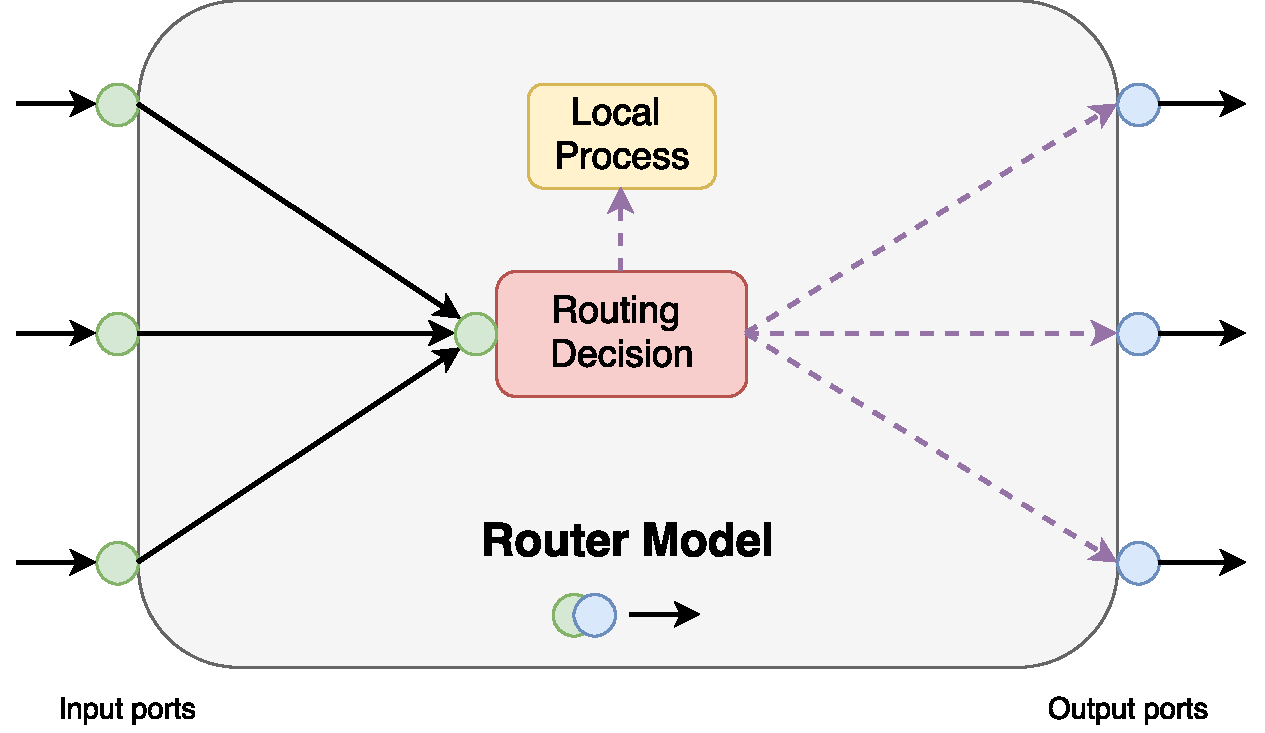
\includegraphics[scale=0.35]{assets/img/router-model}
\end{frame}

\begin{frame}[t]{Towards a Model (2)}
  \begin{itemize}
    \item[2.] Replicate the routing decision element
  \end{itemize}

  \vspace*{0.8cm}

  \centering
  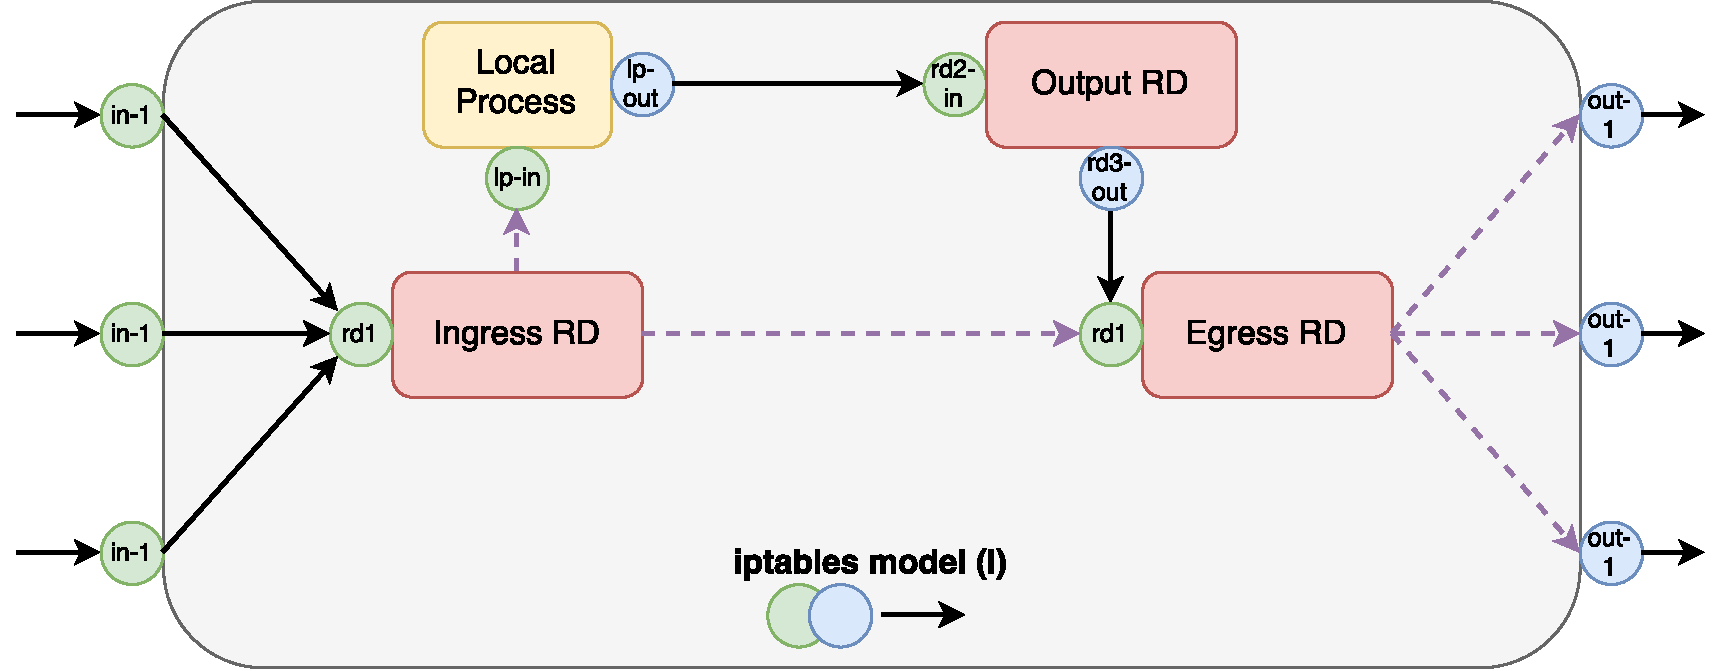
\includegraphics[scale=0.35]{assets/img/iptables-1}
\end{frame}

\begin{frame}[t]{Towards a Model (3)}
  \begin{itemize}
    \item[3.] Abstract each chain as a new \emph{virtual element}
  \end{itemize}

  \vspace*{0.8cm}

  \centering
  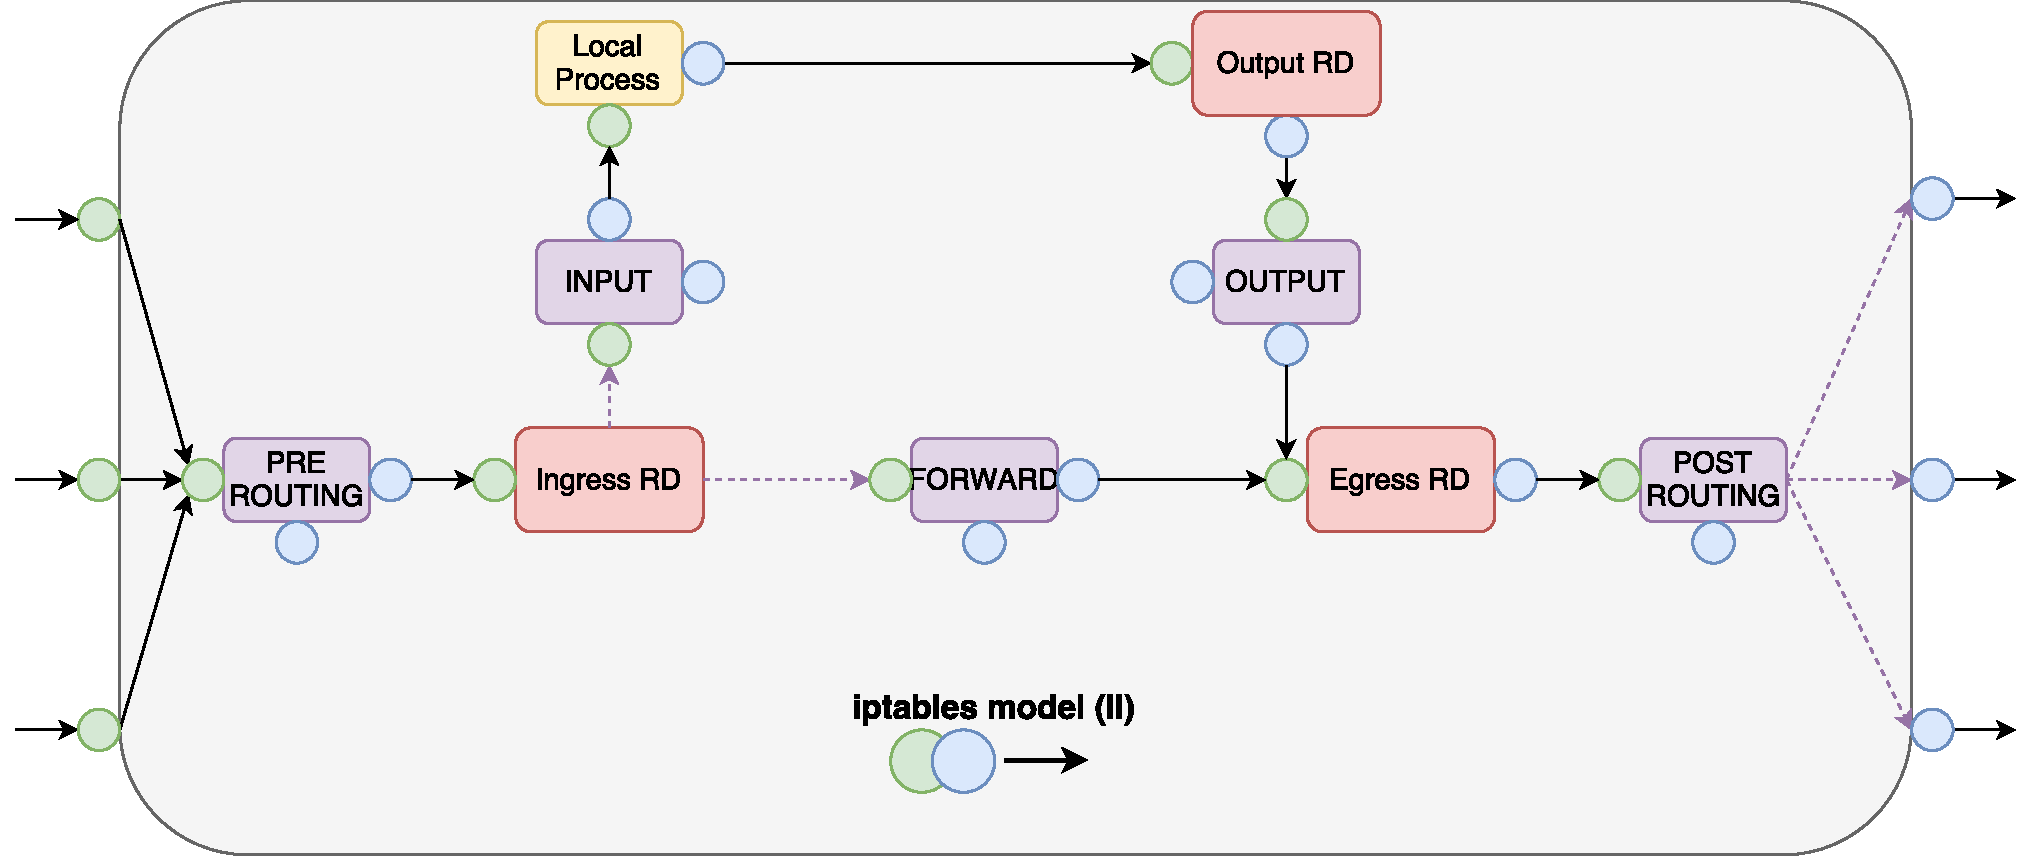
\includegraphics[scale=0.30]{assets/img/iptables-2}
\end{frame}

\begin{frame}{Design and Implementation}
  \begin{itemize}
    \item \emph{iptables-to-sefl}
    \item compiler-like design
      \begin{itemize}
        \item[--] parsing, validation, code generation
      \end{itemize}
    \item extension-oriented
      \begin{itemize}
        \item[--] dynamically enabling match/target extensions
      \end{itemize}
  \end{itemize}

  \centering
  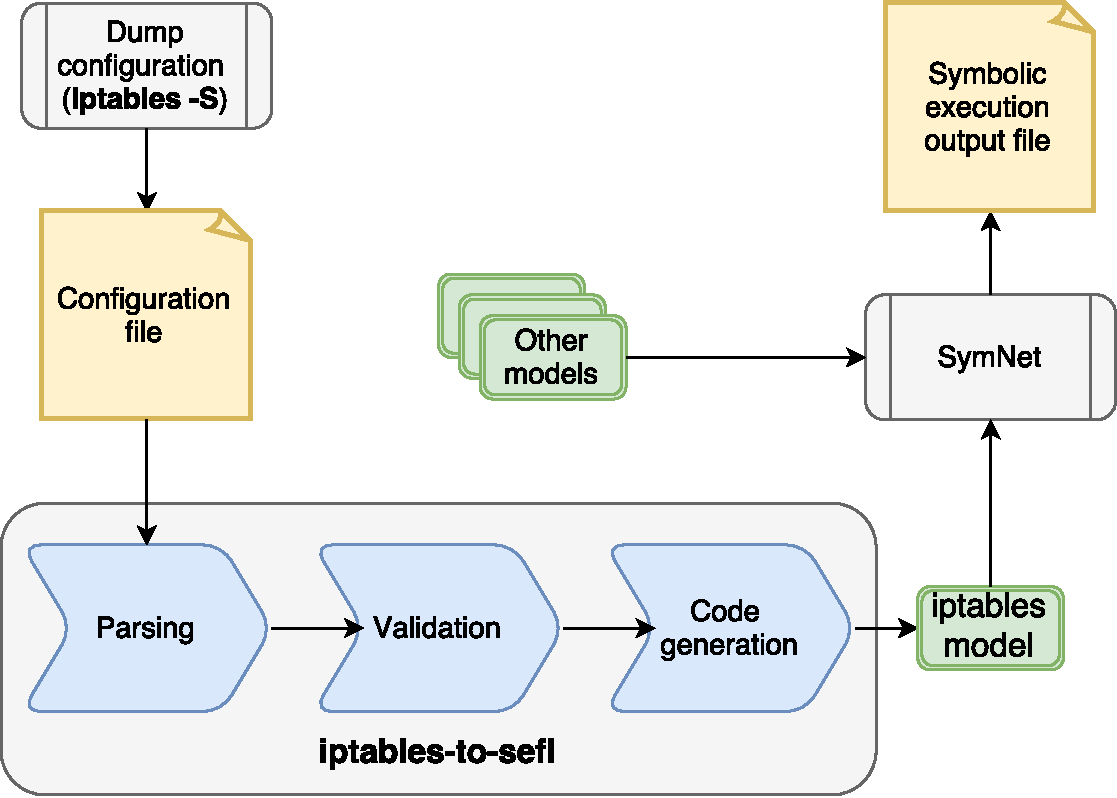
\includegraphics[scale=0.30]{assets/img/high-level-design}
\end{frame}

\begin{frame}{Evaluation - Correctness}
  \begin{itemize}
    \item \emph{Are the resulting models correct?}
    \item Do they capture the iptables semantics they are designed for?

    \vspace*{0.5cm}

    \item Solution: acceptance tests
      \begin{itemize}
        \item[--] ideally, cover all scenarios modelled (i.e. NAT, conntrack,
          jump/return to/from user-chains, etc)
      \end{itemize}
    \item Generic testing topology:
  \end{itemize}

  \vspace*{0.3cm}

  \centering
  \includegraphics[scale=0.40]{assets/img/generic-correctness-testing}
\end{frame}

\begin{frame}{Evaluation - Performance}
  \begin{itemize}
    \item \emph{Are the resulting models fast to verify?}
  \end{itemize}

  \vspace*{0.3cm}

  \begin{columns}
    \begin{column}{.50\textwidth}
      \pgfplotstableread{assets/data/filter-rules.dat}{\rules}
      \pgfplotstableread{assets/data/filter-nat2-rules.dat}{\rulees}
      \pgfplotstableread{assets/data/filter-nat4-rules.dat}{\ruleeees}
      \pgfplotstableread{assets/data/filter-rules-targeted.dat}{\ruls}

      \begin{tikzpicture}[scale=0.72]
        \begin{axis}[
            xmode=log,
            ymin=0,
            ymax=100,
            xlabel=Rules,
            ylabel=Verification time (s),
            ylabel near ticks,
            legend pos=north west,
          ]
          \addplot[mark=*] table [x={rules}, y={time}] {\rules};
          \addlegendentry{filter};

          \addplot[mark=square*,color=red] table [x={rules}, y={time}] {\rulees};
          \addlegendentry{filter+nat(2)};

          \addplot[mark=diamond*,color=blue] table [x={rules}, y={time}] {\ruleeees};
          \addlegendentry{filter+nat(2)+mangle(4)};

          \addplot[mark=triangle*,color=magenta] table [x={rules}, y={time}] {\ruls};
          \addlegendentry{filter (targeted)};
        \end{axis}
      \end{tikzpicture}
    \end{column}
    \begin{column}{.5\textwidth}
      \vspace*{0.15cm}
      \pgfplotstableread{assets/data/network-depth10.dat}{\depthone}
      \pgfplotstableread{assets/data/network-depth20.dat}{\depthtwo}
      \pgfplotstableread{assets/data/network-depth50.dat}{\depthfive}

      \begin{tikzpicture}[scale=0.72]
        \begin{axis}[
            ymin=0,
            ymax=100,
            xlabel=Network depth,
            yticklabels={,,},
            legend pos=north west,
          ]
          \addplot[mark=*,color=black] table [x={depth}, y={time}] {\depthone};
          \addlegendentry{10 rules};

          \addplot[mark=square*,color=red] table [x={depth}, y={time}] {\depthtwo};
          \addlegendentry{20 rules};

          \addplot[mark=triangle*,color=blue] table [x={depth}, y={time}] {\depthfive};
          \addlegendentry{50 rules};
        \end{axis}
      \end{tikzpicture}
    \end{column}
  \end{columns}
\end{frame}

\begin{frame}{Conclusion}
  \begin{itemize}
    % \item What did I do?
    \item iptables-to-sefl: models iptables configurations using SEFL
    \pause
    % \item What did I obtain?
    \item Increased the spectrum of network deployments that can be verified
    \pause
    % \item How good is what I obtained?
    \item Focused on correctness and coverage of commonly used extensions
    \pause
    % \item What is next?
    \item Performance tuning, OpenStack integration
  \end{itemize}
\end{frame}

\begin{frame}{Keywords}
\begin{columns}
  \begin{column}{0.5\textwidth}
    \centering
    \begin{itemize}
      \item network verification
      \item symbolic execution
      \item iptables/netfilter
      \item compiler-like design
      \item extension-oriented
      \item model correctness
    \end{itemize}
  \end{column}
  \begin{column}{0.5\textwidth}
    \centering
    \begin{itemize}
      \item SymNet
      \item SEFL
      \item \emph{iptables-to-sefl}
      \item Scala
    \end{itemize}
  \end{column}
\end{columns}
\end{frame}

\end{document}
